\chapter{Experimental Results}
\label{chap:validation}

\chapter{Experimental Results}
\label{chap:validation}
This chapter presents the evaluation of the key subsystems developed for the GolfBot project. The performance of each component was assessed through a series of quantitative and qualitative tests designed to validate its effectiveness in fulfilling its designated role.

\section{Computer Vision System Evaluation}
\label{sec:cv_evaluation}
The performance of the computer vision system was evaluated in two stages. First, a quantitative analysis of the trained YOLOv11-seg model was conducted using the hold-out test dataset to assess its detection accuracy. Second, a qualitative real-world test was performed to observe the model's robustness in a live operational scenario.

\subsection{Divot Detection Accuracy}
\label{ssec:cv_accuracy}
The accuracy of the trained YOLOv11-seg model was evaluated using standard metrics in the field of object detection. The primary metrics used are Precision (the accuracy of the positive predictions) and Recall (the ability of the model to find all relevant instances).

The relationship between these two metrics is best captured by the Precision-Recall (P-R) curve, shown in Figure \ref{fig:pr_curve}. A model that is close to the top-right corner of the graph maintains high precision even as it finds a high percentage of the true objects (high recall). The area under this curve is summarized by the Mean Average Precision (mAP) score, which is the single most important metric for evaluating object detector performance. As shown in the figure, the model achieved an impressive **mAP@0.5 score of 0.954** across all classes, indicating a high level of accuracy on the test dataset.

\begin{figure}[h!]
    \centering
    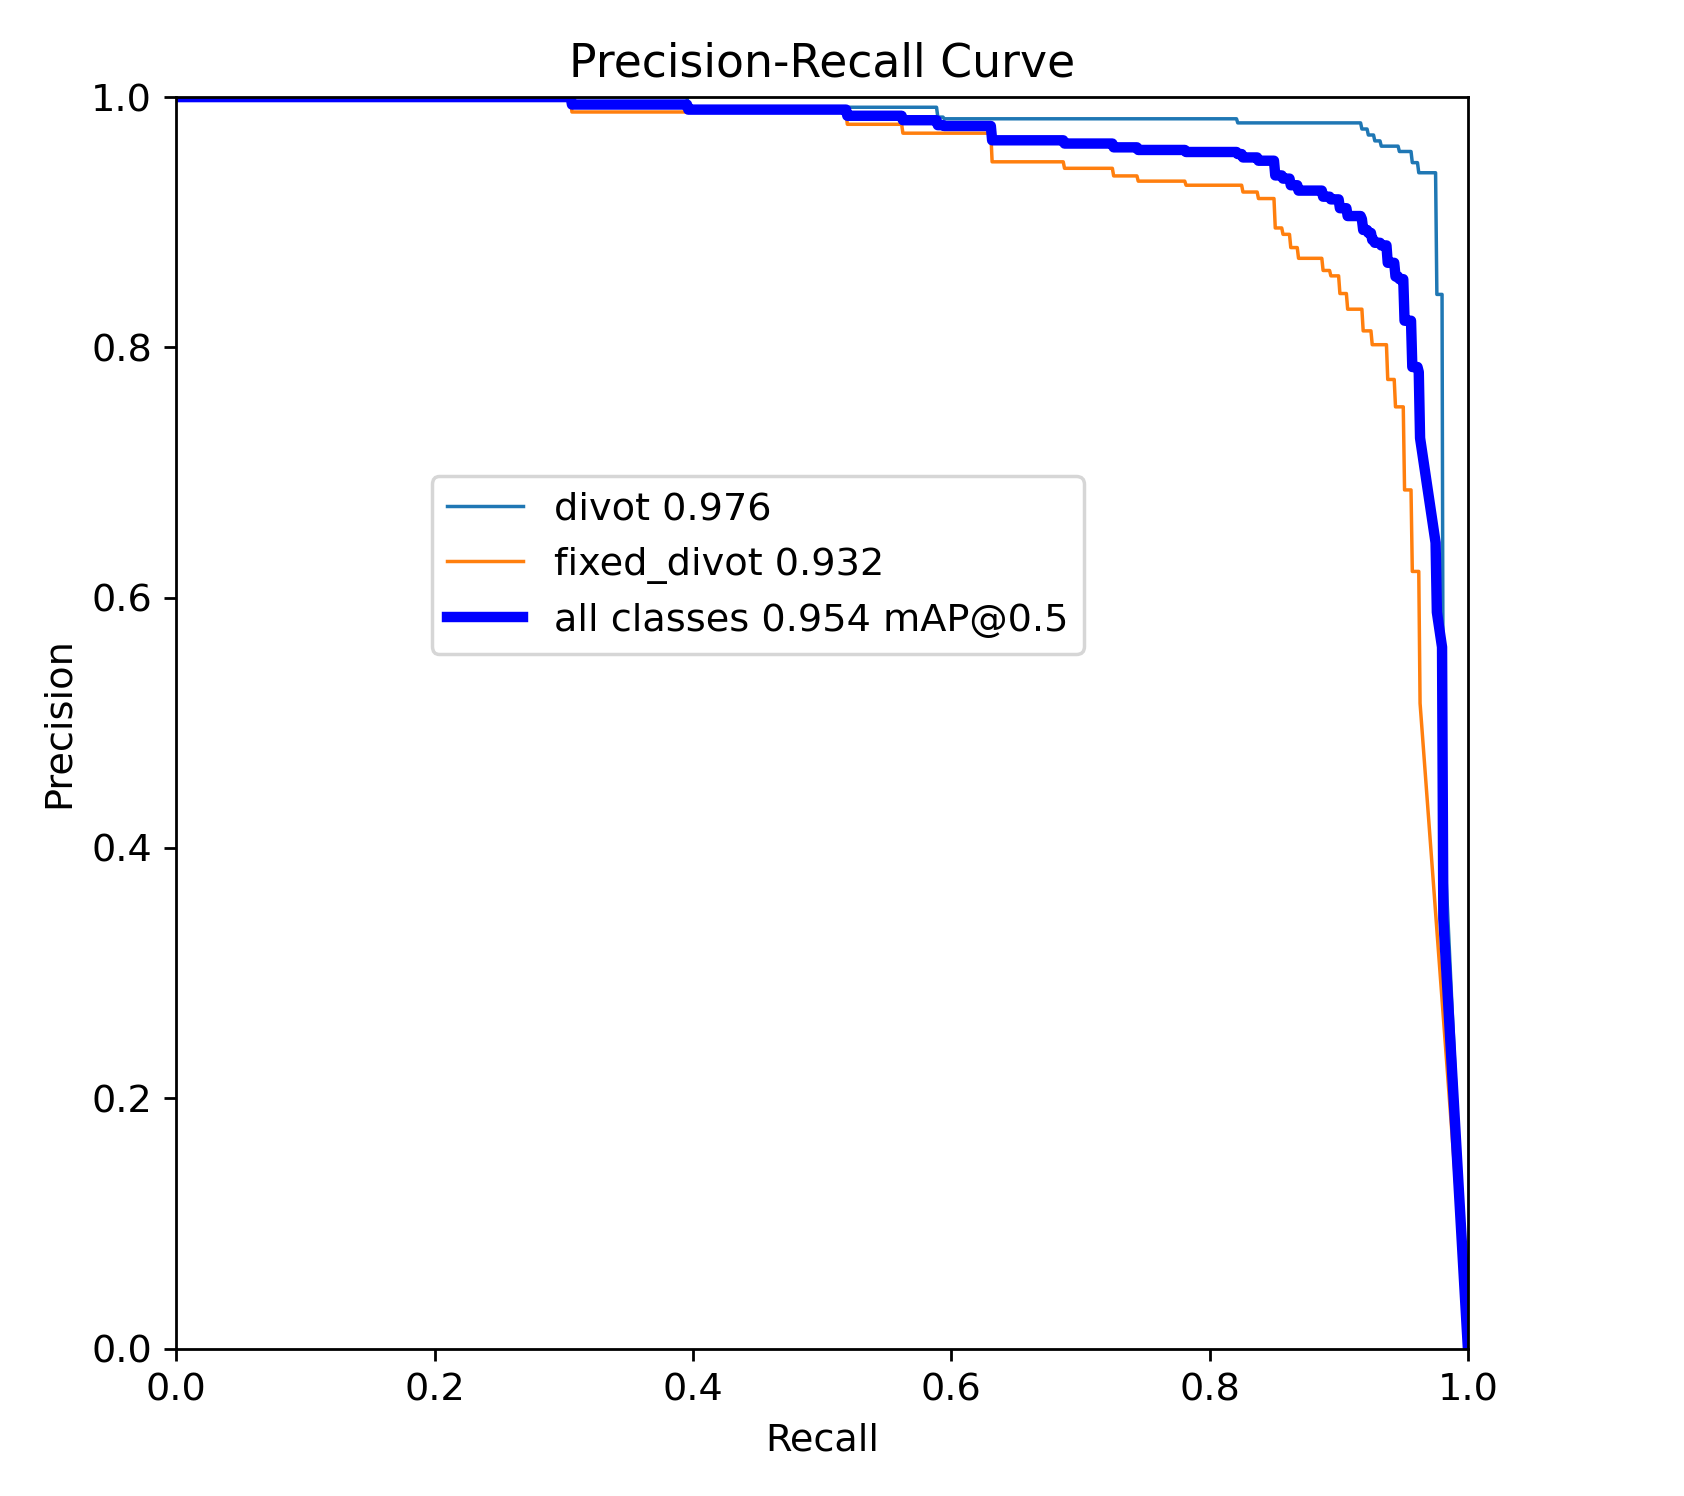
\includegraphics[width=0.8\linewidth]{figures/precision_recall_curve.png}
    \caption{The Precision-Recall (P-R) curve for the trained YOLOv11-seg model. The overall mAP@0.5 of 0.954 demonstrates the model's high accuracy.}
    \label{fig:pr_curve}
\end{figure}

To better understand the model's classification performance, a confusion matrix was generated, as shown in Figure \ref{fig:confusion_matrix}. This matrix shows what categories the model predicted versus the true categories. The normalized version shows that the model is highly effective at its primary task:
\begin{itemize}
    \item It correctly identified true \texttt{divot} instances 98\% of the time.
    \item It correctly identified true \texttt{fixed\_divot} instances 90\% of the time.
    \item The most common error was misclassifying a \texttt{fixed\_divot} as background (10\% of the time), which is an acceptable failure mode as it avoids attempting to repair an already fixed divot.
\end{itemize}

\begin{figure}[h!]
    \centering
    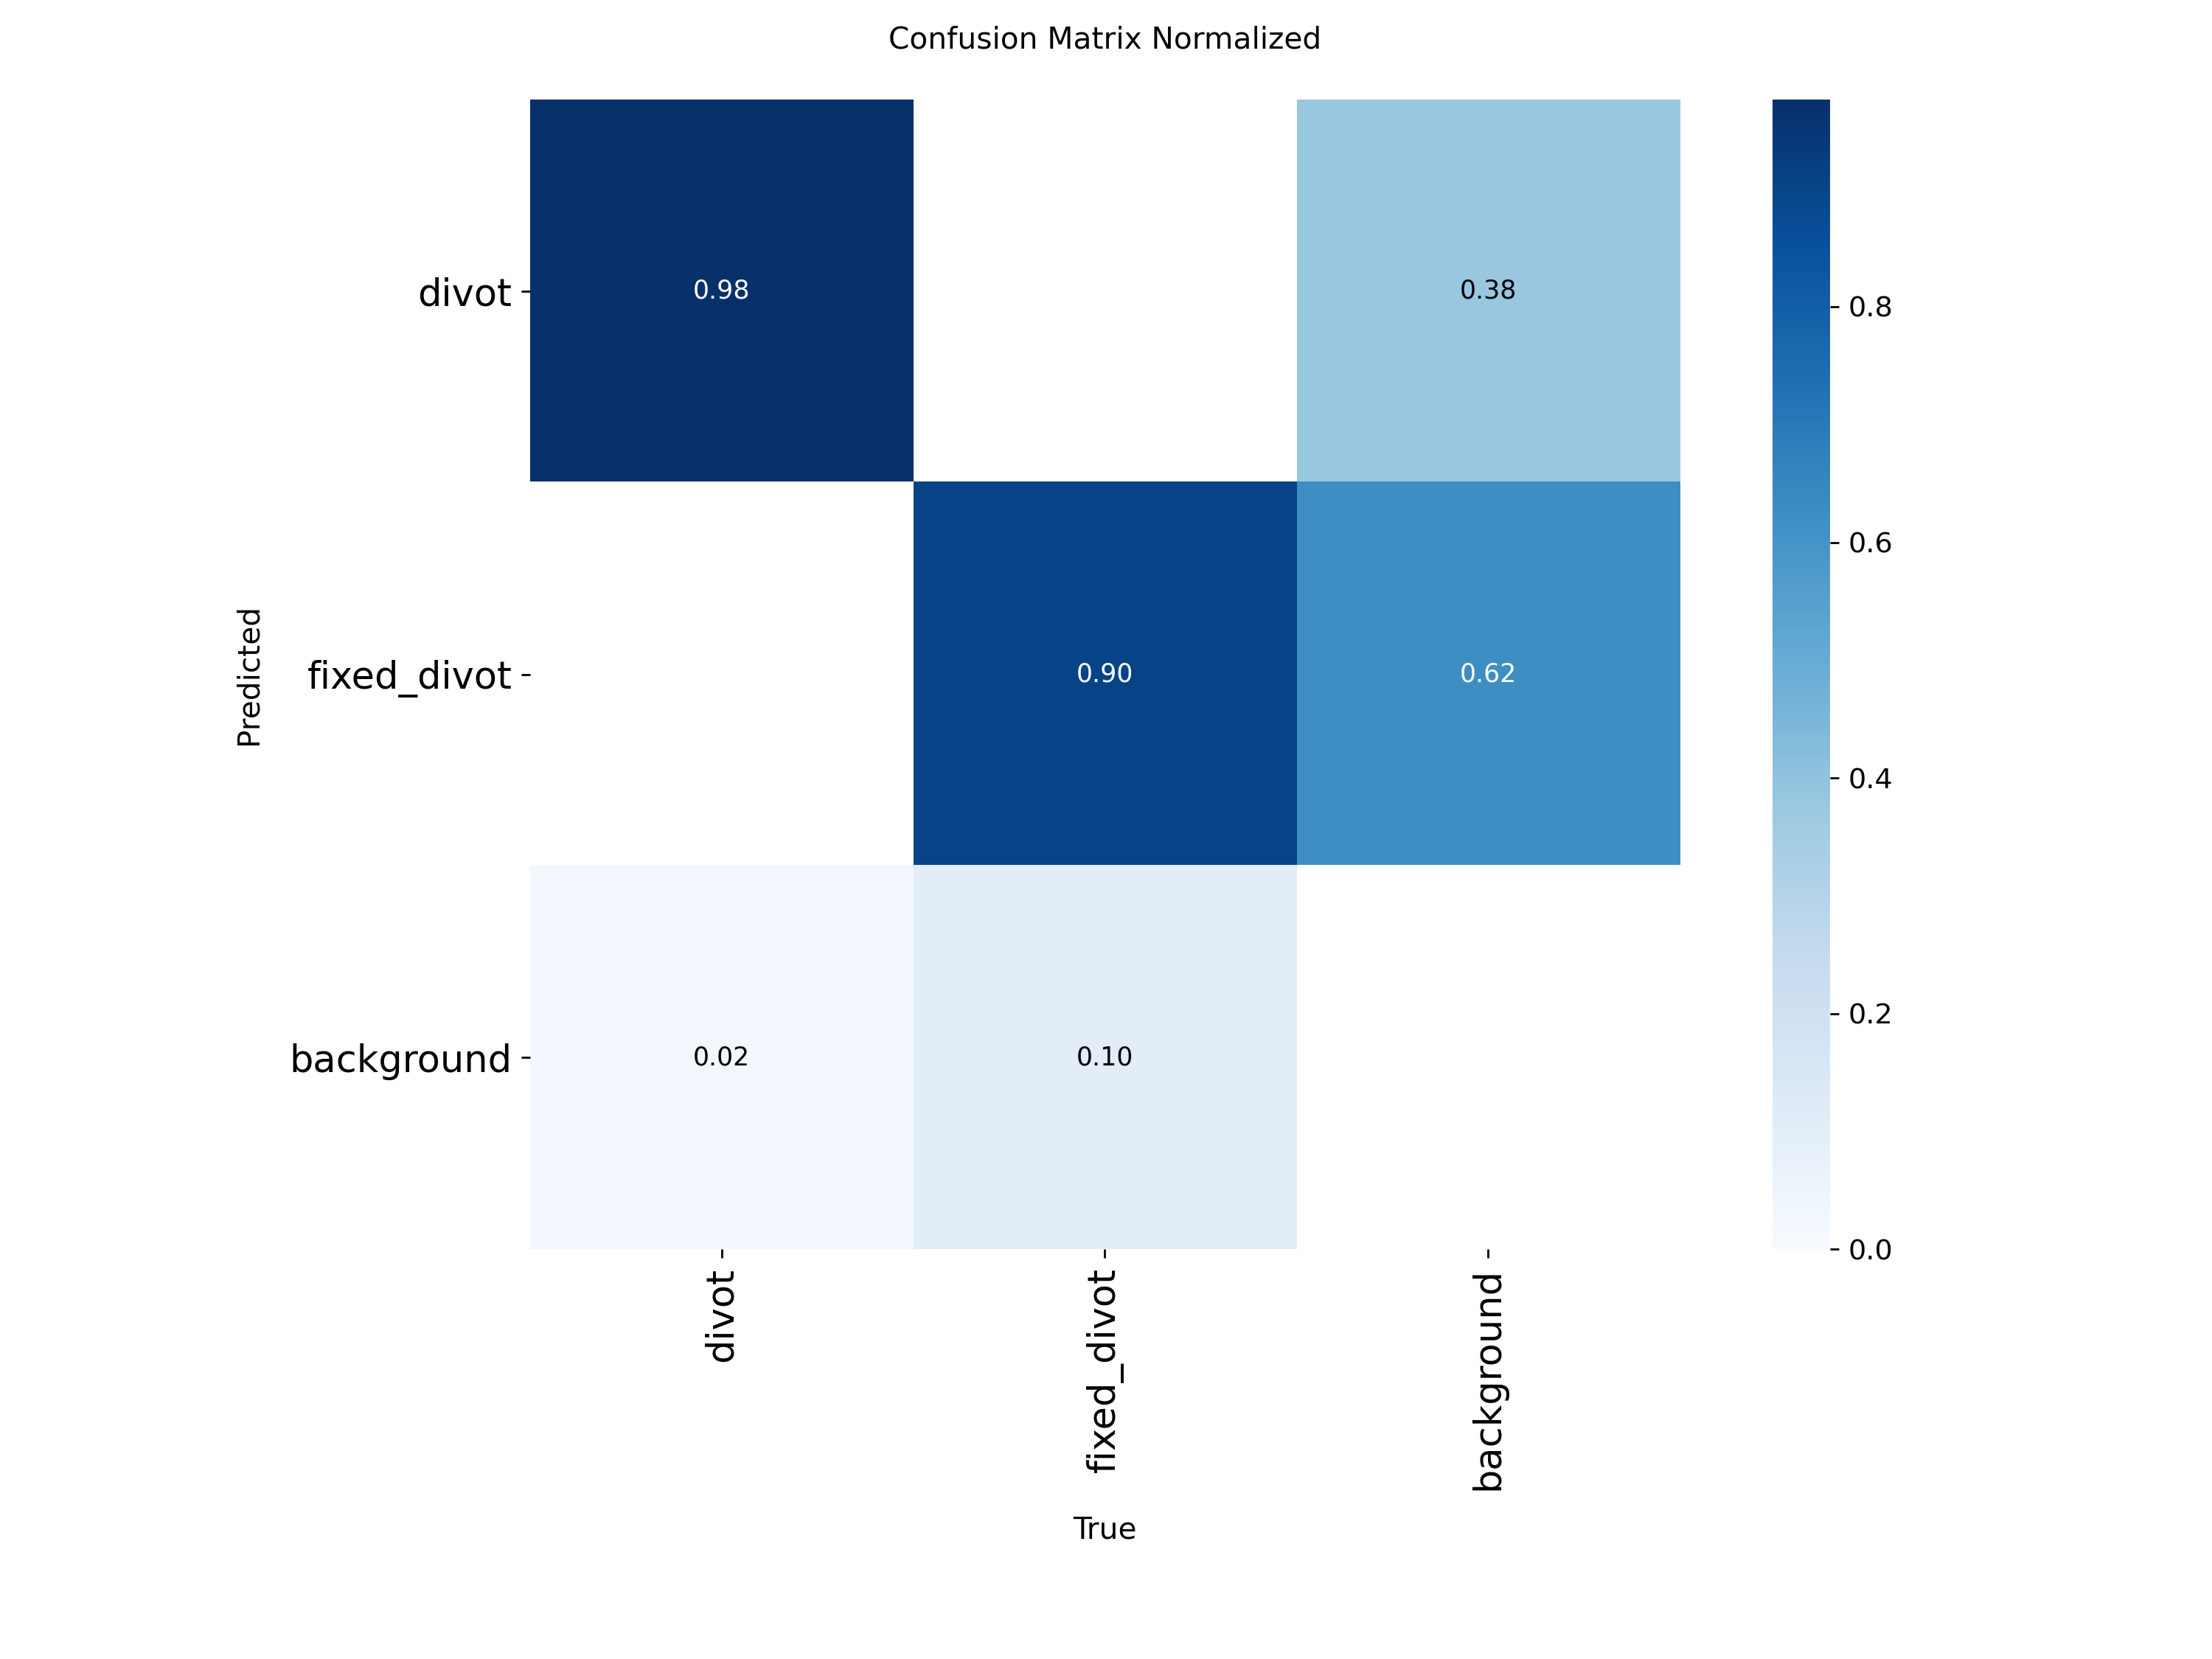
\includegraphics[width=0.7\linewidth]{figures/confusion_matrix_normalized.png}
    \caption{Normalized confusion matrix showing the model's classification accuracy on the test set.}
    \label{fig:confusion_matrix}
\end{figure}

In addition to these quantitative metrics, a qualitative comparison of the model's performance on the unseen validation set is provided in Figure \ref{fig:validation_comparison}. The figure directly compares the ground truth labels (a) with the model's predictions (b) on the same set of images. The high degree of visual similarity between the two provides strong qualitative evidence of the model's effectiveness. The model successfully identifies a variety of divot shapes and sizes under different lighting conditions.

\begin{figure}[h!]
    \centering
    \begin{subfigure}[b]{0.49\textwidth}
        \centering
        \includegraphics[width=\textwidth]{figures/val_batch2_labels.png}
        \caption{Ground truth labels}
        \label{fig:val_labels}
    \end{subfigure}
    \hfill % This creates a small, flexible space between the images
    \begin{subfigure}[b]{0.49\textwidth}
        \centering
        \includegraphics[width=\textwidth]{figures/val_batch2_pred.png}
        \caption{Model's predictions}
        \label{fig:val_preds}
    \end{subfigure}
    \caption{Visual comparison of ground truth labels (a) and the model's predictions (b) on a sample batch of images from the unseen validation set.}
    \label{fig:validation_comparison}
\end{figure}

These quantitative and qualitative results confirm that the model is well-trained and highly capable of distinguishing between divots, fixed divots, and the background environment. Additional performance graphs, including the F1-Confidence curve, are provided in Appendix \ref{chap:appendix_a}.
% \subsection{Real-World Performance}
% \label{ssec:cv_real_world}
% While quantitative metrics validate the model's performance on a static dataset, a qualitative test was conducted to assess its performance in a dynamic, real-world scenario. A full on-course test with the integrated robot was not feasible due to the limitations of the Wumpus platform's wheels, which lacked sufficient traction for consistent navigation on turf.

% Instead, a live test of the vision system was performed. The \texttt{/divot\_detector} ROS 2 node was run on the robot, and the camera was manually pointed at various test subjects in a garden setting that simulated a golf course fairway. This test was designed to evaluate the model's robustness to novel viewpoints, motion blur, and variations in lighting that were not present in the training data.

% The system performed well, successfully identifying and segmenting both new, unseen divots and sand-filled patches in real-time. The visual output from the GUI, as seen in Figure \ref{fig:real_world_examples}, demonstrates the model's ability to generalize to new data. The primary observation was that detection confidence scores tended to be lower in cases of harsh shadows or when a divot was partially obscured by long grass, which is an expected limitation. Overall, this qualitative test confirmed that the implemented computer vision pipeline is robust and suitable for real-world deployment.

% \begin{figure}[h!]
%     \centering
%     \includegraphics[width=\linewidth]{figures/validation_examples.png}
%     \caption{A collage of real-world detection examples from the validation set, showing the model correctly identifying and segmenting both `divot` (blue mask) and `fixed_divot` (cyan mask) instances under various conditions.}
%     \label{fig:real_world_examples}
% \end{figure}

\section{Navigation System Evaluation}
\subsection{Positional Accuracy}
\subsection{Path Following and Search Algorithm Performance}
\subsection{Limitations}

\section{Mechanical Dispenser Evaluation}
\subsection{Dispensing Accuracy and Consistency}

\section{GUI Evaluation}
\subsection{Usability and User Feedback}

\section{Overall Performance of the GolfBot Prototype}
